Lors de cette première étude pilote en présence de comédiens, 
nous avons décidé de se pencher sur le travail d'un monologue en
réalité virtuelle et en particulier sur l'effet de l'environnement 
sur ce travail de monologue. 

Le but de l'étude de ce travail, lors duquel le comédien s'approprie le texte et se plonge dans 
le personnage, est de répondre à plusieurs questions de recherche qui sont les suivantes: 

\begin{itemize}
    \item L'utilisation de l'outil qu'est la réalité virtuelle affecte-t-elle la présence ressentie des comédiens dans leurs roles? Et si oui, comment?
    \item Est-ce que le fait de pouvoir moduler son environnement d'immersion affecte la présence ressentie des comédiens dans leurs roles? Et si oui, quels éléments de l'environnement jouent le plus grand role?
    \item Est ce que le niveau de liberté dans la modulation de cet environnement va avoir un impact sur l'acceptation de ce dernier et sur son influence sur les comédiens? 
\end{itemize}

En partant d'un choix de monologue, le tableau VI de Roberto Zucco de Bernard-Marie
Koltes, nous avons dans un premier temps tiré trois types d'environnements d'immersion 
de nature esthétiques différentes qui permettent d'évaluer quels types de significations 
d'objets vont avoir de l'importance. Les 3 natures esthetiques sont: 
\begin{itemize}
    \item Environnement scénographique: un environnement qui suit les didascalies et qui représente le lieu qui serait représenté sur un plateau
    \item Environnement narratif: un environnement qui illustre les paroles du personnage afin d'immerger le comédien dans son propre récit
    \item Environnement abstrait/émotif: un environnement qui a pour but de susciter chez l'acteur l'état affectif que provoque le sens du texte et son thème 
\end{itemize}

Lors de cette étude, le comédien va pouvoir être en immersion dans 3 environnements différents qui ont été imaginés pour rentrer
dans chacune des ces trois catégories esthétiques. Dans cette scène, Le personnage principal éponyme revendique son invisibilité 
sociale et son conformisme discret, affirmant ne pas être un héros, mais un être ordinaire qui suit sans dévier le cours d'une vie
silencieuse et sans éclat dans l'épais brouillard de la vie. Dans ce contexte la, nous avons modélisé pour la première catégorie, une 
station de métro puisque c'est dans une station de métro que se passe cette scène. Pour la deuxième catégorie, nous avons modélisé un
amphithéatre d'université puisque son monologue évoque sa place dans les rangs des élèves de la Sorbonne. Finalement, pour la troisième 
catégorie, nous avons modélisé un épais brouillard avec une foule de personnages s'affairant autour du comédien pour évoqué le sentiment d'invisibilité dans l'épais brouillard de la vie ordinaire.
Dans ces trois cas, le comédien va soit se voir l'environnement entièrement imposé, soit il aura la possibilité de moduler certains aspects
de celui-ci avec un menu déroulant. En fonction de l'environnement dans lequel il se trouve, l'acteur pourra modifier la taille de la pièce, la luminosité, et
y ajouter et déplacer des objets afin de créer l'espace autour de lui de sorte à ce qu'il fasse écho au sens peronnel du texte qu'il s'approprie. 

\begin{figure}[h]
  \centering

  \begin{minipage}[b]{0.31\textwidth}
    \centering
    \includegraphics[width=\textwidth]{images/metro1.png}
  \end{minipage}
  \hfill
  \begin{minipage}[b]{0.33\textwidth}
    \centering
    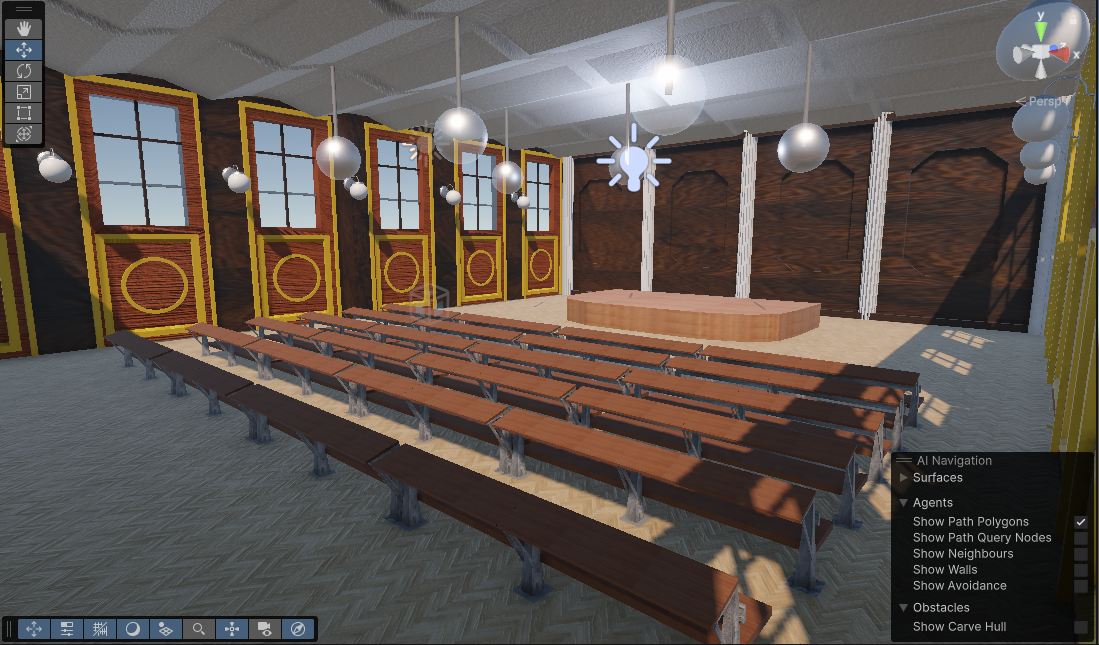
\includegraphics[width=\textwidth]{images/Amphi.png}
  \end{minipage}
  \hfill
  \begin{minipage}[b]{0.32\textwidth}
    \centering
    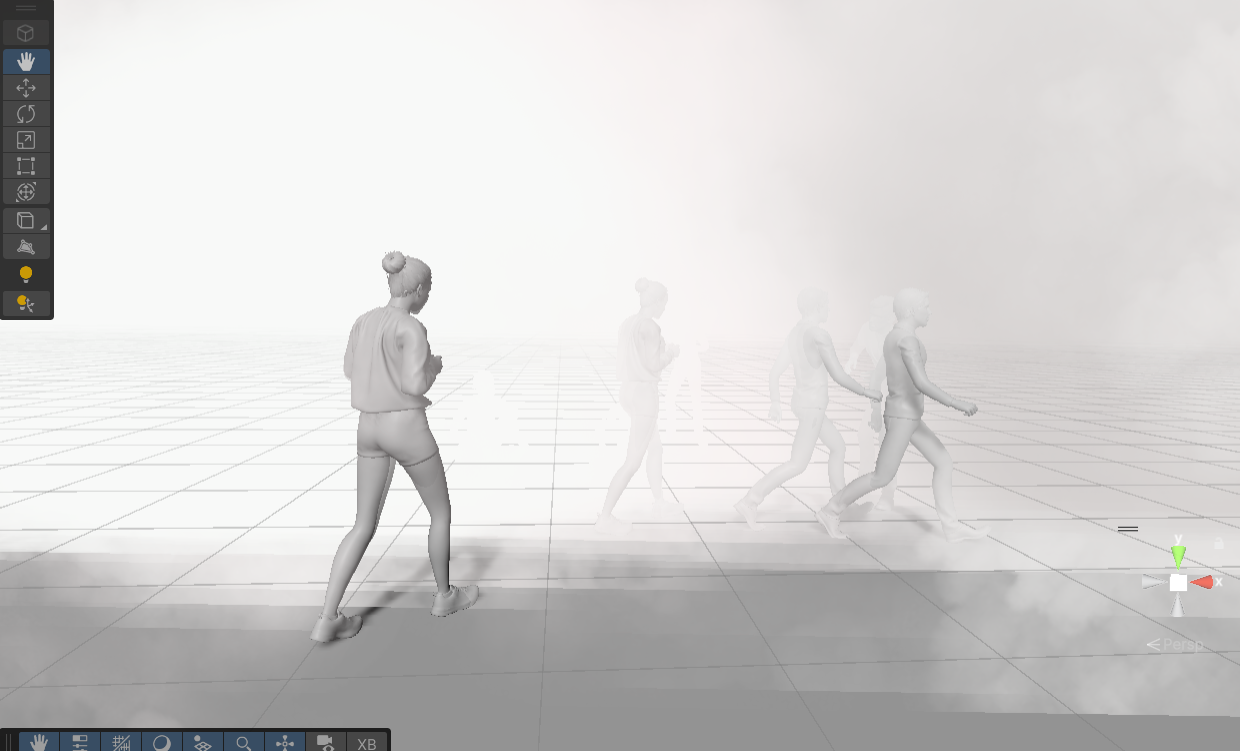
\includegraphics[width=\textwidth]{images/Fog3.png}
  \end{minipage}

  \caption{Captures d'écran des 3 environnements (de gauche à droite: scénographique, narratif, abstrait)}
  \label{fig:trois_images}
\end{figure}
